% josis.tex 1.4   2016-09-15    JoSIS latex template
%------------------------------------------------------------------
% Filename: josis_template.tex
%
% This file is intended as a template for typesetting articles for the
%
%                        Journal of Spatial Information Science.
%
% Please edit this template to generate your own formatted manuscripts
% for submission to JOSIS. See http://josis.org for further details.
%


%%% JOSIS checks in typesetting
%%% * All titles and sections lower case *EXCEPT short title  [ ]
%%% * Remove author postal addresses, only have geographic places and institutions [ ] 
%%% * Consistent use of Section, Figure, Table (capitalized and in full) [ ]
%%% * 10 keywords (and all lower case) [ ]
%%% * Remove all avoidable footnotes [ ]
%%% * Use double quotation marks (``'' not "" or `') [ ]
%%% * Punctuation inside quotations [ ]
%%% * E.g. and i.e. followed by comma [ ]
%%% * cf. followed by tilde [ ]
%%% * Itemize and enumerate correctly punctuated [e.g., "1. x, 2. y, and 3. x." ]
%%% * And/or lists using American English punctuation (e.g., "x, y, and z") [ ] 
%%% * Bibliography (e.g., en-dashes for number ranges, consistent "Proc.~" for Proceedings of..., etc.) []
%%% * Acknowledgment style use section* [ ] 
%%% * et al. no italics, but with dot  [ ] 
%%% * All captions end with full stop  [ ] 
%%% * Table captions under, not over table  [ ]
%%% * Adjust urls with burlalt [ ] 
%%% * Check correct use of hyphens, emdashes, endashes  [ ]
%%% * Perform spell check  [ ] 

%%% JOSIS checks directly before publication 
%%% Check DOI, page numbers on article and web site. [ ]
%%% Update web site with final title, abstract, keywords. [ ] 
%%% Build with distiller for DOI links. [ ]


% Required documentclass definition for JOSIS
\documentclass{josis}
\usepackage{hyperref}
\usepackage[hyphenbreaks]{breakurl}
\usepackage{booktabs}
\usepackage{stmaryrd}
\usepackage[T1]{fontenc}
\usepackage{cite}

% Suggested packages for algorithm formatting
\usepackage{algorithm}
%\usepackage{algorithmic}
\usepackage{algpseudocode}


\usepackage[table]{xcolor}
\usepackage{amssymb,amsmath}

\renewcommand{\topfraction}{0.9} 
\renewcommand{\textfraction}{0.1}

% Page setup and overhangs
\sloppy
\widowpenalty=10000
\clubpenalty=10000
\hyphenpenalty=75

% Article details for accepted manuscripts will be added by editorial staff
% Omit year if article in press
% Omit number if article under review
\josisdetails{%
   number=N, year=YYYY, firstpage=xx, lastpage=yy, 
  doi={10.5311/JOSIS.\textit{TBD}},
   received={December 18, 2024}, 
   returned={\textit{TBD}},
   revised={},
   accepted={}, }

\newcommand{\mydoi}[1]{\href{http://dx.doi.org/#1}{doi:\protect\detokenize{#1}}}

%\renewcommand{\UrlLeft}{http:\sslash}
%\DeclareUrlCommand\myurl{\def\UrlLeft{}\def\UrlRight{}%
%\urlstyle{tt}}

\urlstyle{rm}
\makeatletter
% Inspired by http://anti.teamidiot.de/nei/2009/09/latex_url_slash_spacingkerning/
% but slightly less kern and shorter underscore
\let\UrlSpecialsOld\UrlSpecials
\def\UrlSpecials{\UrlSpecialsOld\do\/{\Url@slash}\do\_{\Url@underscore}}%
\def\Url@slash{\@ifnextchar/{\kern-.11em\mathchar47\kern-.2em}%
    {\kern-.0em\mathchar47\kern-.08em\penalty\UrlBigBreakPenalty}}
\def\Url@underscore{\nfss@text{\leavevmode \kern.06em\vbox{\hrule\@width.3em}}}
\makeatother

\hypersetup{
colorlinks=true,
linkcolor=black,
citecolor=black,
urlcolor=black
} 

% Add the running author and running title information
\runningauthor{\begin{minipage}{.9\textwidth}\centering Julian Kraft\end{minipage}}
\runningtitle{Wildlife sightings WebApp}

% Document begins
\begin{document}
%\setcounter{page}{33}


% Insert your own title
\title{A Web Application for Wildlife Sightings - how accessible is this technology using modern frameworks?}

% Insert your manuscipts authors, affiliations, and addresses
\author{Julian Kraft}\affil{LSFM, ZHAW, Switzerland}

\maketitle

% Add 5-10 keywords for every submission
\keywords{Web Application, Wildlife Sightings, Geodata, Field Recording, Web Frameworks}

% Add a short abstract of 150-250 words
\begin{abstract}
The aim of this semester project is to assess the accessability of the technology to create a web application to record geo tagged data.
With the help of modern web frameworks, a web application was built to record wildlife sightings. A working prototype was created and and made
available online with the option to install it on smartphones of all major operating systems.
The project was a success and the technology is accessible to everyone with a bit more than basic programming knowledge, some help and some 
insane persistence.

\end{abstract}

% Your main text begins here. 
\section{Introduction}

At the heart of any project involving geospatial data are the data themselves. If these data are not yet available, 
the goal is to find an appropriate method to collect them. In the field of environmental sciences, 
data collection still often relies on manual methods. However, this fieldwork can also be simplified through the use of technology. 
A suitable tool for this purpose is something almost everyone possesses -- a smartphone.
A quick online search reveals that there are already many apps available that can accomplish this. 
However, these are often relatively expensive, offer far more features than actually needed, 
and control over the data often lies with the app provider. With all the modern frameworks 
and programming languages available today, it should not be that difficult to write a 
custom app that does exactly what is required.
And so, the idea to create a custom app was born.
In this case an example to record wildlife sightings was chosen as the use case.
The general idea is to create an individual toolkit from wich future use cases can be derived. 
This work aims to examine just how challenging it really is to develop an app, 
particularly with very limited prior knowledge, a lot of trial and error, 
extensive research, the use of AI, immense patience, 
and a bit to significantly more support from an experienced developer.

It was with this support that the project began. To avoid having to figure everything out from scratch, 
the process started with a consultation. During this meeting, the idea was presented, 
and discussions were held on which technologies, programming languages, 
and frameworks would be practical, feasible, and sensible. 
In a subsequent session, the server was configured, and the development environment was set up together. 
A not-so-small crash course then provided a solid foundation for diving into the project.

\section{Methods}

The app essentially consists of three parts: the web-based frontend, the backend server, 
and the database. These three components are interconnected and communicate with each other. 
The frontend is the user interface displayed on the smartphone, 
the backend handles the logic running in the background, 
and the database serves as the storage location for all data that is retrieved or saved.

\subsection{Frontend}

The frontend was created using the Ionic framework. Ionic is an open-source toolkit for 
developing mobile user interfaces. It is based on Angular, another open-source framework developed by Google. 
Ionic enables the creation of web applications that run on all platforms -- Android, iOS, and web -- while 
offering native app-like performance and experience \cite{IonicFrameworkCrossPlatform}.
The framework makes it relatively easy to start a project and test it in a development environment, 
where the app is displayed in the browser. The actual programming is done using the programming 
languages HTML, CSS, and TypeScript. TypeScript is a programming language developed by Microsoft that is based on JavaScript. 
CSS is a stylesheet language used for designing the user interface, while HTML is a markup language used for structuring the user interface.

\subsection{Backend}

The backend was created using the programming language Go. Go is a programming language developed 
by Google that is used for the development of web applications and servers. 
It is easy to learn and use and offers good performance \cite{GoProgrammingLanguage}.
It is also worth mentioning that GitHub Copilot provides excellent suggestions for 
the Go programming language, which significantly simplifies programming. The main logic handled 
by the backend in the app includes user authentication, accessing the database to check for available 
users or retrieve options for animals, and transforming and saving new data in the database.

\subsection{Database}

The database used is MariaDB. MariaDB is a relational database derived from MySQL and developed by the open-source community. 
It is easy to install and use and offers good performance \cite{MariaDBFoundation}.
In this case, Docker was used to install the database on the server and run it in a so-called container. 
The database consists of three tables: \texttt{users}, \texttt{tierarten}, and \texttt{sichtungen}, 
where \texttt{tierart\_id} and \texttt{user\_id} are used as foreign keys in the \texttt{sichtungen} table. 
The ER diagram of the database is shown in Figure~\ref{fig:db_structure}.

\begin{figure}[tbh]
    \centering
    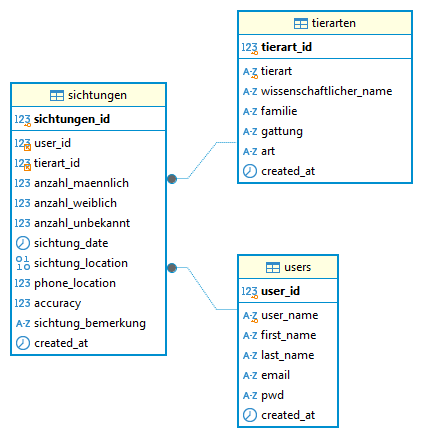
\includegraphics[width=0.6\textwidth]{images/db_structure.png}
    \caption{ER Diagram of the database}\label{fig:db_structure}
\end{figure}

\subsection{WebMap}

A final component used in the app is a WebMap. This is retrieved directly from the frontend 
via Google Web Services and embedded into the app. To enable this, 
a Google developer account is required to create a WebMap, 
which can then be accessed using a MapID. Configurations regarding the appearance of the map can be made directly in the Google developer account.

\subsection{Design}

The design of the app is really quite simple. In general it just uses the default styling of the Ionic framework with very minor adjustments.
The only patt where some effort was put in was the logo. The logo was designed by a fellow student and is shown in Figure~\ref{fig:logo}.
The idea is to vertically show the general purpose of recording geo tagged data. Horizontally it symbolizes the data content of the app.
So for future use cases the logo can be easily adjusted to fit the new content.
\begin{figure}[tbh]
    \centering
    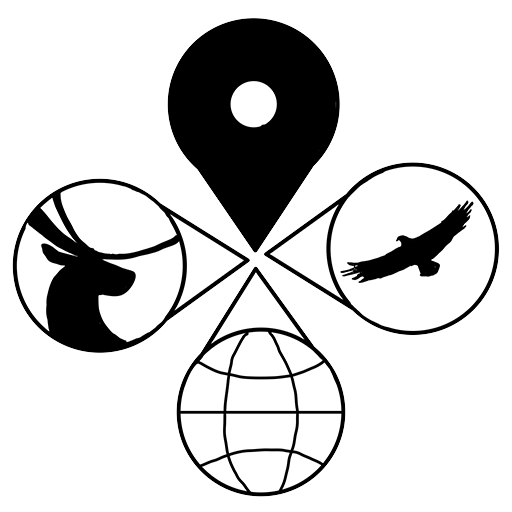
\includegraphics[width=0.4\textwidth]{images/logo_app.png}
    \caption{Logo for the app}\label{fig:logo}
\end{figure}

\section{Results}

\subsection{Web Application}

The app was successfully developed and deployed. And will be available for a few months after the submission of this report.
It seems a bit pointless to describe the app in detail here, as it is available online and can be tested by anyone.
To install the app on a smartphone just use the qr code in Figure~\ref{fig:qr_code_app} or visit 
the website \url{https://wildtierapp.juliankraft.ch/app/}. On opening the page a prompt will suggest the installation of the app.
It works best using the Google Chrome browser. In order for the app to work, location services must be enabled on the smartphone
and the app must be granted access to the location.

\begin{figure}[tbh]
    \centering
    
\includegraphics[width=0.3\textwidth]{images/qr_code_app.png}
    \caption{QR Code to install the app}\label{fig:qr_code_app}
\end{figure}

\subsection{Data View}

In addition to the app, a data view was created to display the data collected by the app. It is publicly available and can be 
accessed at \url{https://wildtierapp.juliankraft.ch/}. This works best using the Google Chrome browser on a computer.

\subsection{Data Access}

This data view is only a frontend to display the data. In order to access the data for further processing, a REST API was created.
A python script to access the data and a config file for a read only user is available on the GitHub repository 
for the backend under \path{./db_setup/}.
Feel free to use this script to and config file to access the data for testing. However the data is not valid since it was created for testing purposes only
and anyone testing the app can add random data to the database.

\subsection{Code Base}
All the code for the app is publicly available on GitHub:
\begin{itemize}
    \item Frontend: \url{https://github.com/juliankraft/WildtierSichtungsApp_front}
    \item Backend: \url{https://github.com/juliankraft/WildtierSichtungsApp_back}
\end{itemize}

It is worth mentioning that the code is not perfect -- at this point it is not more than a working prototype. Still the code is open source and can
be used by anyone to do whatever under the creative commons license CC0 1.0 Universal.

\section{Discussion}

\section*{Acknowledgments}

I would like to express my gratitude to Ramon Ott -- the experienced developer -- for his help and support during this project. 
Without his help, this project would not have been possible.
I very much appreciate the help of my fellow student Annalisa Berger for her great work on the design of the logo for the application.

\section*{Declarations}

The creation of this document was supported by ChatGPT and GitHub Copilot. 
Additionally, AI played a significant role in the development of the prototype.
The Introduction and the Methods section where translated from German to English using
ChatGPT since they where written before realizing that this report had to follow the JOSIS template
specifically defining the language.

\bibliographystyle{josisacm}
\bibliography{josisexample}

\end{document}